\documentclass{article}
\usepackage{amsmath}
\usepackage{amssymb}
\usepackage{graphicx}
\usepackage{hyperref}
\usepackage[version=4]{mhchem}

\title{Problem 8}
\date{}

\begin{document}
\maketitle

\section*{Problem}
As shown in the figure, \(A B\) and \(C D\) are diameters of the circle \(O . A B\) and \(C D\) are perpendicular. \(\angle C D F=30^{\circ}\). Chord \(D F\) intersects \(A B\) at \(E\) with \(D E=10\) and \(E F=5\). Find the area of the circle.\\
(A) \(25 \pi\)\\
(B) \(\frac{75}{2} \pi\)\\
(C) \(75 \pi\)\\
(D) \(\frac{95}{2} \pi\)\\
(E) \(95 \pi\)\\
\centering
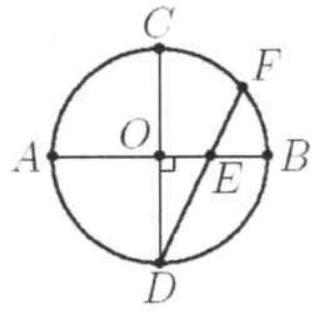
\includegraphics[width=\textwidth]{images/problem_image_1.jpg}

\section*{Solution}
(C).\\
Connect \(C F\). Angle \(C F D\) forms a right angle and \(C D F\) is a \(30^{\circ}-60^{\circ}-90^{\circ}\) right triangle. It follows that the ratio of the sides is \(1: \sqrt{3}: 2\).\\
Since \(D F=10+5=15, C F=5 \sqrt{3}=r\). The area is \(\pi r^{2}=\)\\
\centering
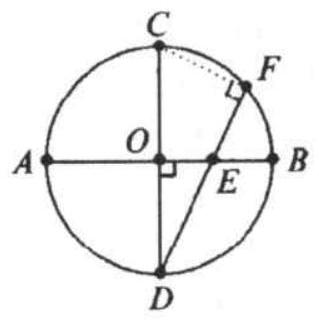
\includegraphics[width=\textwidth]{images/reasoning_image_1.jpg}


\(\pi(5 \sqrt{3})^{2}=75 \pi\).

\end{document}
